%%____________________________________________________________________________||

\section{\texorpdfstring{\znunu\ + jets}{Zinv} background estimation}
\label{sec:zinv}

The irreducible background contribution from the \znunu\ + jets
process can be a sizeable, and often the dominating, contribution in
many event categories of the signal region, as illustrated by
Fig.~\ref{fig:breakdownmc} in Sec.~\ref{sec:smbreakdown}, and
particularly at high \HTmiss.

The method to estimate the \znunuj background is very similar to that
used for the lost lepton background estimate described in
Sec.~\ref{sec:ttw}, as it is based on the use of transfer factors as
well as templates taken from simulation that are validated against
control region data. However, there are some minor differences, which
are described below. 

%\fixme{Diff w.r.t. old analysis. Heavy flavour.}

\subsection{The ``transfer factor'' method}
\label{sec:tf-method-zinv}

As for the lost lepton background estimate described in
Sec.~\ref{sec:tf-method-ttw}, the method used to estimate the \znunuj
background also relies on the use of transfer factors determined from
simulated event samples. 

The categorisation of events according to \njet in the \mmj control
region is identical to that in the signal region, and the
categorisation according to \scalht is very similar.\footnote{Again,
  as for the lost lepton background method, the predictions are based
  on the \scalht categorisation used in the control regions (up to 11
  bins) and aggregated over a range in \scalht to map onto a coarser
  binning scheme that is used in the signal region (up to 5
  bins). Further details can be found in
  Sec.~\ref{sec:ht-categorisation}.} With regards to \nb, the \mmj
event sample is subdivided as follows, $\nb = 0$ and $\nb \geq 1$, as
outlined in Sec.~\ref{sec:nb-categorisation}. For the former
subsample, no extrapolation in \nb is performed when predicting the
\znunuj background in the corresponding (\njet, \scalht, $\nb = 0$)
bin of the signal region. However, for the latter subsample, counts in
data and from simulation for the \mmj control region are integrated
for the region $\nb \geq 1$. These integrated counts are used to
predict the \nb distribution (for the region $\nb \geq 1$ only) in the
signal region using \nb templates obtained from simulation per (\njet,
\scalht) bin. The extrapolation in \nb is validated through control
region studies, as described in Sec.~\ref{sec:nb-zinv}.

The transfer factors and predictions for the \znunuj background are
defined as follows:
\begin{eqnarray}
  \label{equ:tf-ratio-zinv}
  {\rm TF} & = &   
  \frac{N_{\rm MC}^{\znunu}(\njet, \scalht, \nb)}
  {N_{\rm MC}^{\mmj}(\njet, \scalht, \nb)} \\
  \npre^{\znunu}(\njet, \scalht, \nb) & = &
  {\rm TF}
  \times 
  \nobs^{\mmj}(\njet, \scalht, \nb)   
\end{eqnarray}
where $N_{\rm MC}^{\mmj}$ and $\nobs^{\mmj}$ reflect counts in regions
defined by $\nb = 0$ and $\nb \geq 1$.

The selection criteria for the \mmj control region
(Sec.~\ref{sec:selection}) closely resemble those for the signal
region, differing mainly through the requirement of a dimuon system
and minimal additional kinematic requirements, such as a dimuon
invariant mass requirement compatiable with the mass of the Z
boson. These criteria provide a sample enriched in \zmmj events and
depleted in signal and multijet events. Any signal contamination is
accounted for in the likelihood model (Sec.~\ref{sec:likelihood}).

Figure~\ref{fig:tf_mmZinv} (App.~\ref{app:zinv}) shows the magnitude
of the transfer factors, typically $>1$, The transfer factors account
for differences between the \mmj control and signal due to the
different branching fractions for the decays to neutrinos or muons, as
well as differences in acceptance times efficiency for the
reconstructed muons and extrapolations in kinematic quantities. As for
the \mj sample, the dependence on \njet and \scalht is largely
attributable to the \alphat and \bdphi requirements for the signal
region (that are not used in the \mmj control region).

Systematic uncertainties are assigned to the transfer factors to
account for theoretical uncertainties as well as effects such as the
mismodelling of kinematics (\eg acceptances) and instrumental effects
(\eg reconstruction efficiencies). These uncertainties are discussed
below.

\subsection{\texorpdfstring{\mht}{MHT} templates}
\label{sec:mht-zinv-intro}

As discussed above, the \mmj events are categorised similarly to
candidate signal events in terms of \njet, \scalht, and \nb. However,
no categorisation of \mmj events is performed as a function of \mht,
which is used in the signal region to discriminate effectively between
SM background and \eg a potential contribution from SUSY processes.

An \mht template per (\njet, \scalht, \nb) category is used, which is
equivalent to dicing the numerator of the transfer factor according to
\mht. Hence, the transfer factors can be written as:
\begin{equation}
  \label{equ:pred-method-zinv-mht}
  \npre^{\znunu}(\njet, \scalht, \HTmiss, \nb) = 
  \frac{N_{\rm MC}^{\znunu}(\HTmiss;\; \njet, \scalht, \nb)}
  {N_{\rm MC}^{\mj}(\njet, \scalht, \nb)} 
  \times 
  \nobs^{\mj}(\njet, \scalht, \nb)
\end{equation}

In this regard, the TFs described in Sec.~\ref{sec:tf-method-zinv}
provide an estimate of the normalisation for each \mht template. The
\HTmiss templates are taken from simulation and the validity of the
simulation modelling is tested extensively in the control regions, as
described in Sec.~\ref{sec:mht-zinv}.

\subsection{Sideband normalisation for \texorpdfstring{\zj}{Z+jets}} 
\label{sec:sideband-corrections-zinv}

Corrections to the inclusive cross section used for the \zmmj
simulated samples are determined following a procedure that uses a
binned likelihood fit to data in \HTmiss sidebands of the \mj and \mmj
control regions. Correspondingly, the same corrections are applied to
the \znunuj simulated samples. The procedure is defined in
Sec.~\ref{sec:sideband-corrections}.

As noted previously, this iteration of the analysis is {\em not}
sensitive to whether these corrections are applied or not, due to the
way the transfer factors are constructed. Contrary to the previous
iteration of this analysis, only the \zmmj sample is now used to
predict the \znunuj background.\footnote{In the previous iteration of
  the analysis, all three control regions (\mj, \mmj, and \gj) were
  used to predict the \znunu\ background.} The corrections and
uncertainties for the \zmmj and \znunuj processes, as determined by
the fit, are shown in Table~\ref{tab:sbCorrsFromFit-zinv}.

\begin{table}[!h]
%  \scriptsize
  \centering
  \topcaption{Corrections to the inclusive cross sections 
    for the \zmmj and \znunuj processes determined from a binned
    likelihood fit to data in the $100 < \HTmiss < 200\GeV$ sideband
    to the control regions.}
  \label{tab:sbCorrsFromFit-zinv}
  \begin{tabular}
    {clc}
    \hline
    \textbf{Process} & \textbf{Sample} & \textbf{Corrrection} \\
    \hline
%    \zmmj            & \mmj            & $1.06 \pm 0.01$      \\ % no NLO/NISR
    \zmmj            & \mmj            & $0.91 \pm 0.01$      \\
    \znunuj          & (\mmj as proxy) & $0.91 \pm 0.01$      \\
    \hline
  \end{tabular}
\end{table}


\subsection{Overview of systematic uncertainties}
\label{sec:systematics-zinv}

The following sections address the estimation of systematic
uncertainties related to the \znunuj background estimation. All
relevant uncertainties are listed in Table~\ref{tab:systs-zinv}, along
with their representative magnitudes and assumptions on inter-bin
correlations. How the uncertainties are incorporated into the
likelihood model is described in Sec.~\ref{sec:likelihood}.

\begin{table}[h!]
  \caption{Sources of systematic uncertainty in the transfer factors
    used to estimate the \znunuj background using the \mmj control
    region. Also shown are the nuisance parameters and correlation
    scheme, as well as representative ranges for the uncertainties
    [\%]. The representative range is taken from the $16\%$ and $84\%$
    percentiles on the transfer factor variations across all analysis
    bins for each source of systematic. The ``type'' refers to whether
    the nuisance parameters are unique to the \znunuj background or
    shared with the lost lepton background estimate
    (see Table~\ref{tab:systs-ttw}).
  }
  \label{tab:systs-zinv}
  \centering
  \fontsize{8}{9.6}\selectfont
  \newcommand{\cat}{\njet, \scalht, \nb, \mht}
  \begin{tabular}{ llllc }
    \hline
    Source of uncertainty               & Nuisance parameters / correlation   & Magnitude (\%)                       & Shared & Figure                              \\
    \hline
    Finite-size simulated samples       & 1 per (\cat) category               & 1--100                               & Unique & n/a                                 \\
    Minimum bias cross section (pileup) & 1, correlated across \cat           & 2.3--2.8                             & Shared & \ref{fig:tfSyst_pu_mmZinv}          \\
    $\mu_R$ / $\mu_F$ scales            & 1, correlated across \cat           & 0.9--4.7                             & Shared & \ref{fig:tfSyst_scale_mmZinv}       \\
    Parton density functions            & 1, correlated across \cat           & 0.0--3.3                             & Shared & \ref{fig:tfSyst_pdf_mmZinv}         \\
    QCD + EWK NLO corrections           & 1, correlated across \cat           & 2.2--14.3                            & Shared & \ref{fig:tfSyst_nlo_mmZinv}         \\
    Signal trigger efficiency           & 1, correlated across \cat           & 0.0--2.0                             & Shared & \ref{fig:tfSyst_trigger_mmZinv}     \\
    Lepton efficiency (selection)       & 1, correlated across \cat           & 0.0--4.2                             & Unique & \ref{fig:tfSyst_muonsf_mmZinv}      \\
    Jet energy scale                    & 1, correlated across \cat           & 5.3--8.0                             & Shared & \ref{fig:tfSyst_jec_mmZinv}         \\
    b-quark tag efficiency              & 1, correlated across \cat           & 0.3--0.6                             & Shared & \ref{fig:tfSyst_bsf_mmZinv}         \\
    b-quark mistag probability          & 1, correlated across \cat           & 0.2--1.8                             & Shared & \ref{fig:tfSyst_bsfl_mmZinv}        \\
    \alphat extrapolation               & 1 per \njet, 1 per \scalht category & 3.3--9.4 (\njet), 2.1--5.9 (\scalht) & Unique & \ref{fig:closure_AlphaT_mumu}       \\
    \bdphi extrapolation                & 1 per \njet, 1 per \scalht category & 2.7--22. (\njet), 1.6--18. (\scalht) & Unique & \ref{fig:closure_bDPhi_mumu}        \\
%    Single isolated track veto          & 1 per \njet, 1 per \scalht category & 0.0--0.3 (\njet), 0.0--0.3 (\scalht) & Unique & \ref{fig:closure_SITV_mumu}         \\
    \hline
  \end{tabular}
\end{table}

Several sources of uncertainty are evaluated.  The most relevant
effects are discussed below, and generally fall into one of two
categories. The first category concerns known theoretical and
experimental effects that are propagated through to the transfer
factors and \HTmiss templates. These are decribed in
Sec.~\ref{sec:mc-variations-zinv}. The second set can be considered as
``known unknowns'' that are derived from dedicated ``closure test''
and \HTmiss-modelling studies that involve confronting transfer
factors determined in the phase space of this search against data in
the control regions. This latter category of uncertainties are
summarised in Secs.~\ref{sec:closure-tests-zinv} and
\ref{sec:mht-zinv}.

\subsection{Known theoretical and experimental uncertainties}
\label{sec:mc-variations-zinv}

Most of the uncertainties considered for the determination of the lost
lepton background, described in Sec.~\ref{sec:mc-variations} are also
considered here. The same treatment and assumptions are made. Below,
we simply highlight relevant behvaviours and reference the
corresponding figures. 

\subsubsection{Minimum bias cross section / pileup}
\label{sec:tfSyst_pu-zinv}

The relative change in the transfer factors under this variation is
small, at the few percent level, as shown in
Fig.~\ref{fig:tfSyst_pu_mmZinv} (App~\ref{app:zinv}).

\subsubsection{Effect of scale and PDF on lepton acceptance}
\label{sec:tfSyst_pdf-zinv}

Figures~\ref{fig:tfSyst_scale_mmZinv} and \ref{fig:tfSyst_pdf_mmZinv}
(App.~\ref{app:zinv}) show the behaviour in the transfer factors for
variations in scale and PDF, respectively.

\subsubsection{Missing higher-order corrections in LO \texorpdfstring{\MADGRAPH}{MadGraph}
  samples}
\label{sec:nlo-zinv}

The \zmmj and \znunuj processes are generated at leading order with
the \MADGRAPH code. The effect of missing higher-order QCD and EWK
corrections are studied by considering the effect of
LO$\rightarrow$NLO corrections, determined as a function of Z boson
\Pt and shown in in Fig.~\ref{fig:tfSyst_nlo_mmZinv}
(App.~\ref{app:zinv}), on the transfer factors and \HTmiss templates.
Fig.~\ref{fig:NLO_app} (App.~\ref{app:ttw}) then show the effects of the NLO
corrections on the event yield in each bin in the Signal Region.
These corrections include
NLO QCD corrections derived using {\MADGRAPH{}5\_a\MCATNLO},
and NLO electroweak corrections derived from theoretical calculations,
as described in Ref.~\cite{monojet_AN_36fb}.

Simulated \zmmj and \znunuj events are weighted according to these NLO
corrections, and the magnitude of each correction is propagated as an
uncertainty throughout the analysis. Fig.~\ref{fig:tfSyst_nlo_mmZinv}
(App.~\ref{app:zinv}) show the effect on the transfer factors as a
function of the various discriminating variables. Uncertainties are
typically at the percent level and as large as $\sim 15\%$.

\subsubsection{Signal trigger uncertainty}
\label{sec:tfSyst_trigger-zinv}

The relative change in the transfer factors is typically at the few
percent level, as presented in Fig.~\ref{fig:tfSyst_trigger_mmZinv}
(App~\ref{app:zinv}).

\subsubsection{Lepton trigger / identification / isolation efficiencies}
\label{sec:leptonSyst-zinv}

Figure~\ref{fig:tfSyst_muonsf_mmZinv} (App.~\ref{app:zinv}) shows the
systematic uncertainties associated with the data/simulation scale
factors related to the trigger, identification, and isolation
efficiencies for muon selection.

\subsubsection{Jet energy scale}
\label{sec:tfSyst_jec-zinv}

The relative change in the transfer factors is presented as a function
of \scalht and jet category in Fig.~\ref{fig:tfSyst_jec_mmZinv}
(App.~\ref{app:zinv}). The changes are typically in the range of
$5-8\%$.

\subsubsection{B-tagging efficiency and mistag probability}
\label{sec:tfSyst_btag-zinv}

The relative change in the transfer factors is presented as a function
of \scalht and jet category in Figs.~\ref{fig:tfSyst_bsf_mmZinv} and
\ref{fig:tfSyst_bsfl_mmZinv} (App.~\ref{app:zinv}).  They are
typically in the range of $0-2\%$.

\subsection{Systematics uncertainties in transfer factors from closure tests}
\label{sec:closure-tests-zinv}

As described in Sec.~\ref{sec:closure-tests}, a second category of
uncertainty is determined from sets of closure tests based on data
control samples~\cite{RA1Paper2012}. The tests relevant to the \znunuj
background estimate are listed below. 

\subsubsection{Extrapolation in \texorpdfstring{\alphat}{AlphaT} and
  \texorpdfstring{\bdphi}{biased dPhi}}
\label{sec:tfSyst_alphaT-zinv}

Events in the \mmj control region are not required to satisfy any
requirement on \alphat or \bdphi. Hence, the accuracy of the modelling
of the the \alphat and \bdphi variables are estimated using the \mmj
sample using dedicated closure tests that confront data yields in a
subsample of \mmj events, satisfying the \alphat and/or \bdphi
requirements, against predictions that are determined using another
subsample of \mmj events that satisfy an inverted requirement on
\alphat and/or \bdphi. Further details of the procedure are found in
Sec.~\ref{sec:closure-tests}. 

The level of closure for an extrapolation in \alphat (only) with the
\mmj sample is shown in Fig.~\ref{fig:closure_AlphaT_mumu}
(App.~\ref{app:zinv}) as function of \scalht and \njet. Similarly,
Fig.~\ref{fig:closure_bDPhi_mumu} (App.~\ref{app:zinv}) shows the same
information for the extrapolation in \bdphi (only). 
%Finally, the level of closure observed when both \alphat and \bdphi
%requirements are simultaneously imposed is summarised in
%Fig.~\ref{fig:closure_AlphaT_bDPhi_mumu} (App.~\ref{app:zinv}).

Any non-closure in the extrapolation of both \alphat and \bdphi is
covered by a systematic uncertainty, which is defined as the
quadrature sum of the observed non-closure and its statistical
uncertainty (indicated by the blue histogram in the figures). 

\subsection{Systematic uncertainties in the \texorpdfstring{\HTmiss}{MHT} templates}
\label{sec:mht-zinv}

The modelling of the \mht variable for the \znunuj background is
performed with the \mmj sample as a proxy. Discussion and motivation
for these tests of the \mht modelling against data are provided in
Sec.~\ref{sec:mht}. Here, for brevity, only the figures are
summarised.

The figures in App.~\ref{app:mht-zinv} show the ratio of events
obtained from data and simulation as a function of \mht based on a
sample of \mmj events that are {\it categorised} according to \njet,
\scalht, and \nb. Note that the \scalht categorisation scheme of the
control regions (Sec.~\ref{sec:ht-categorisation}) is used in this
validation of the \mht modelling. The \nb categorisation is not
relevant for this discussion.

\begin{figure}[h!]
  \centering
  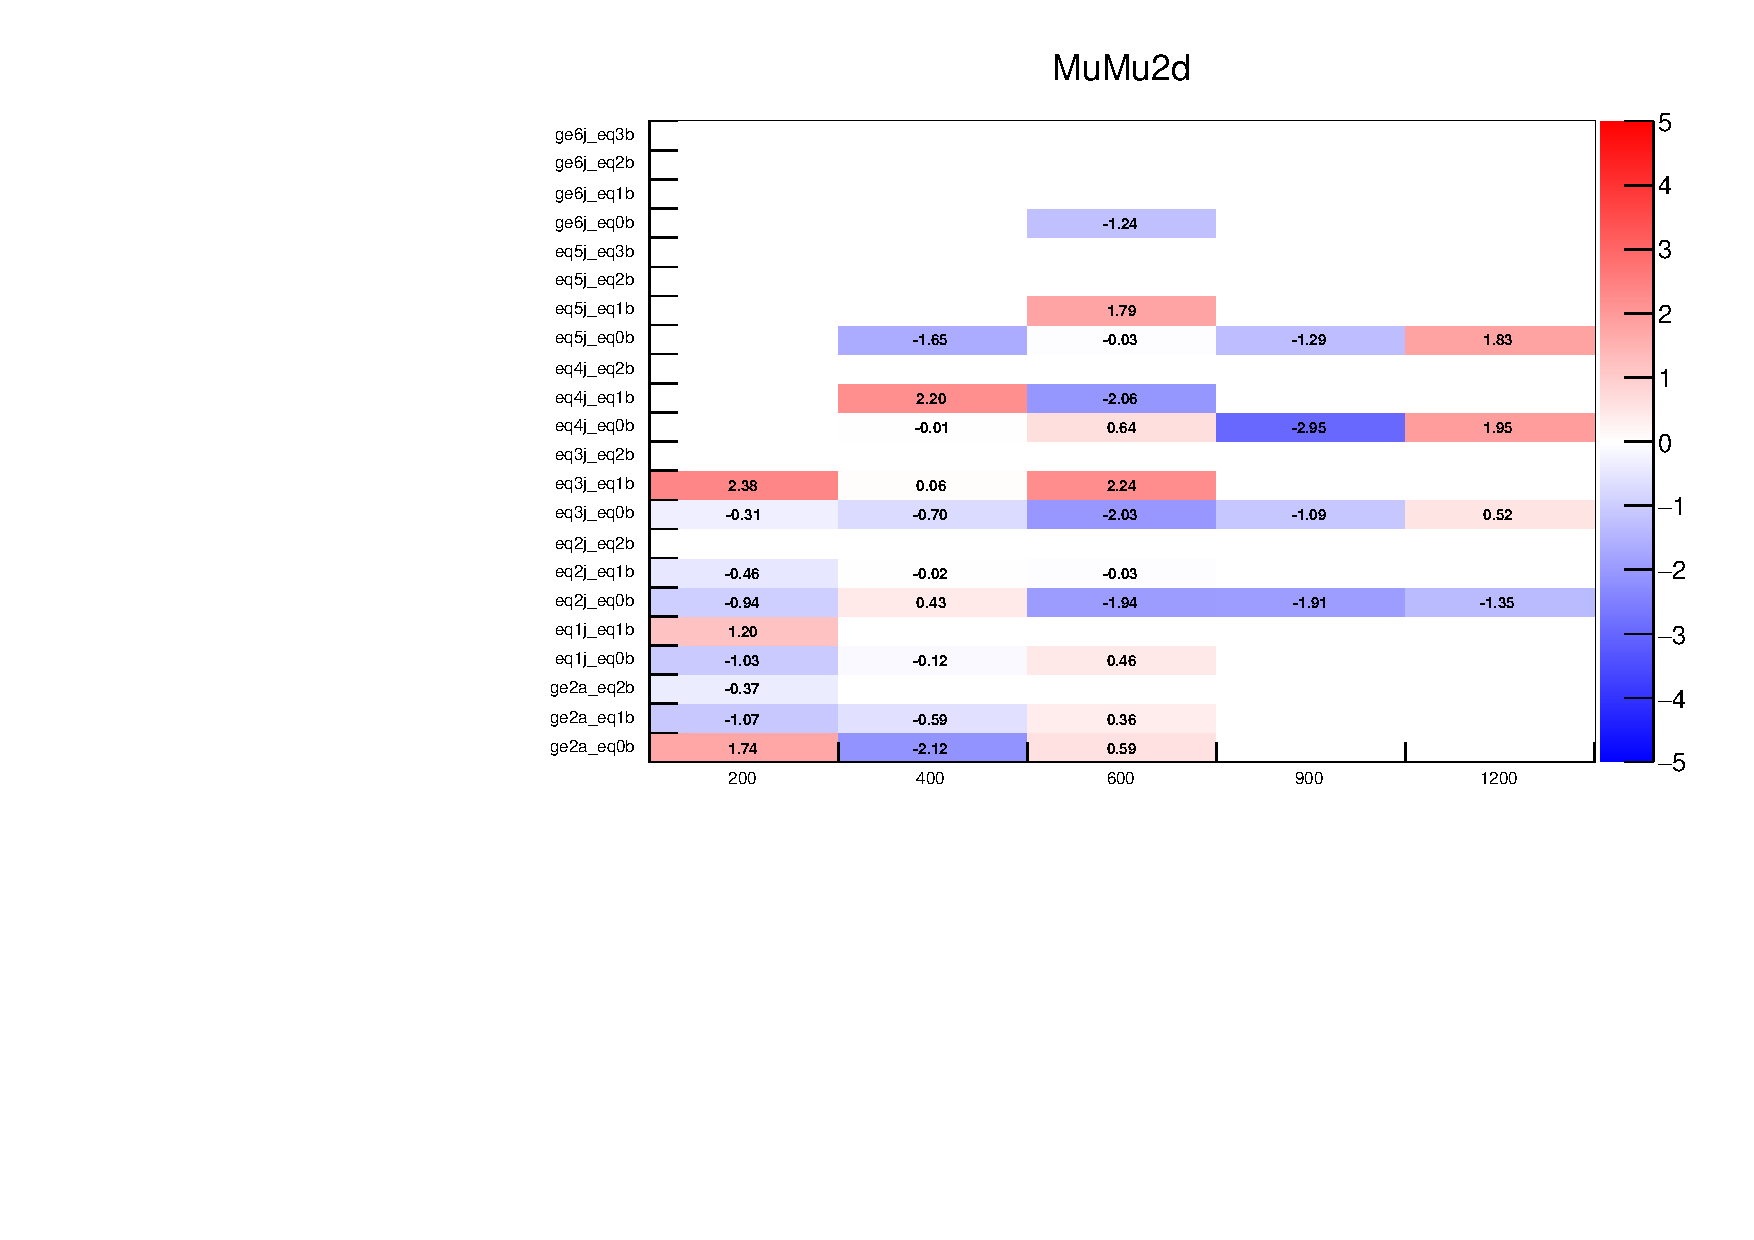
\includegraphics[width=0.5\textwidth]{figures/mhtTemplate/exclusive/MuMu_2D}~
  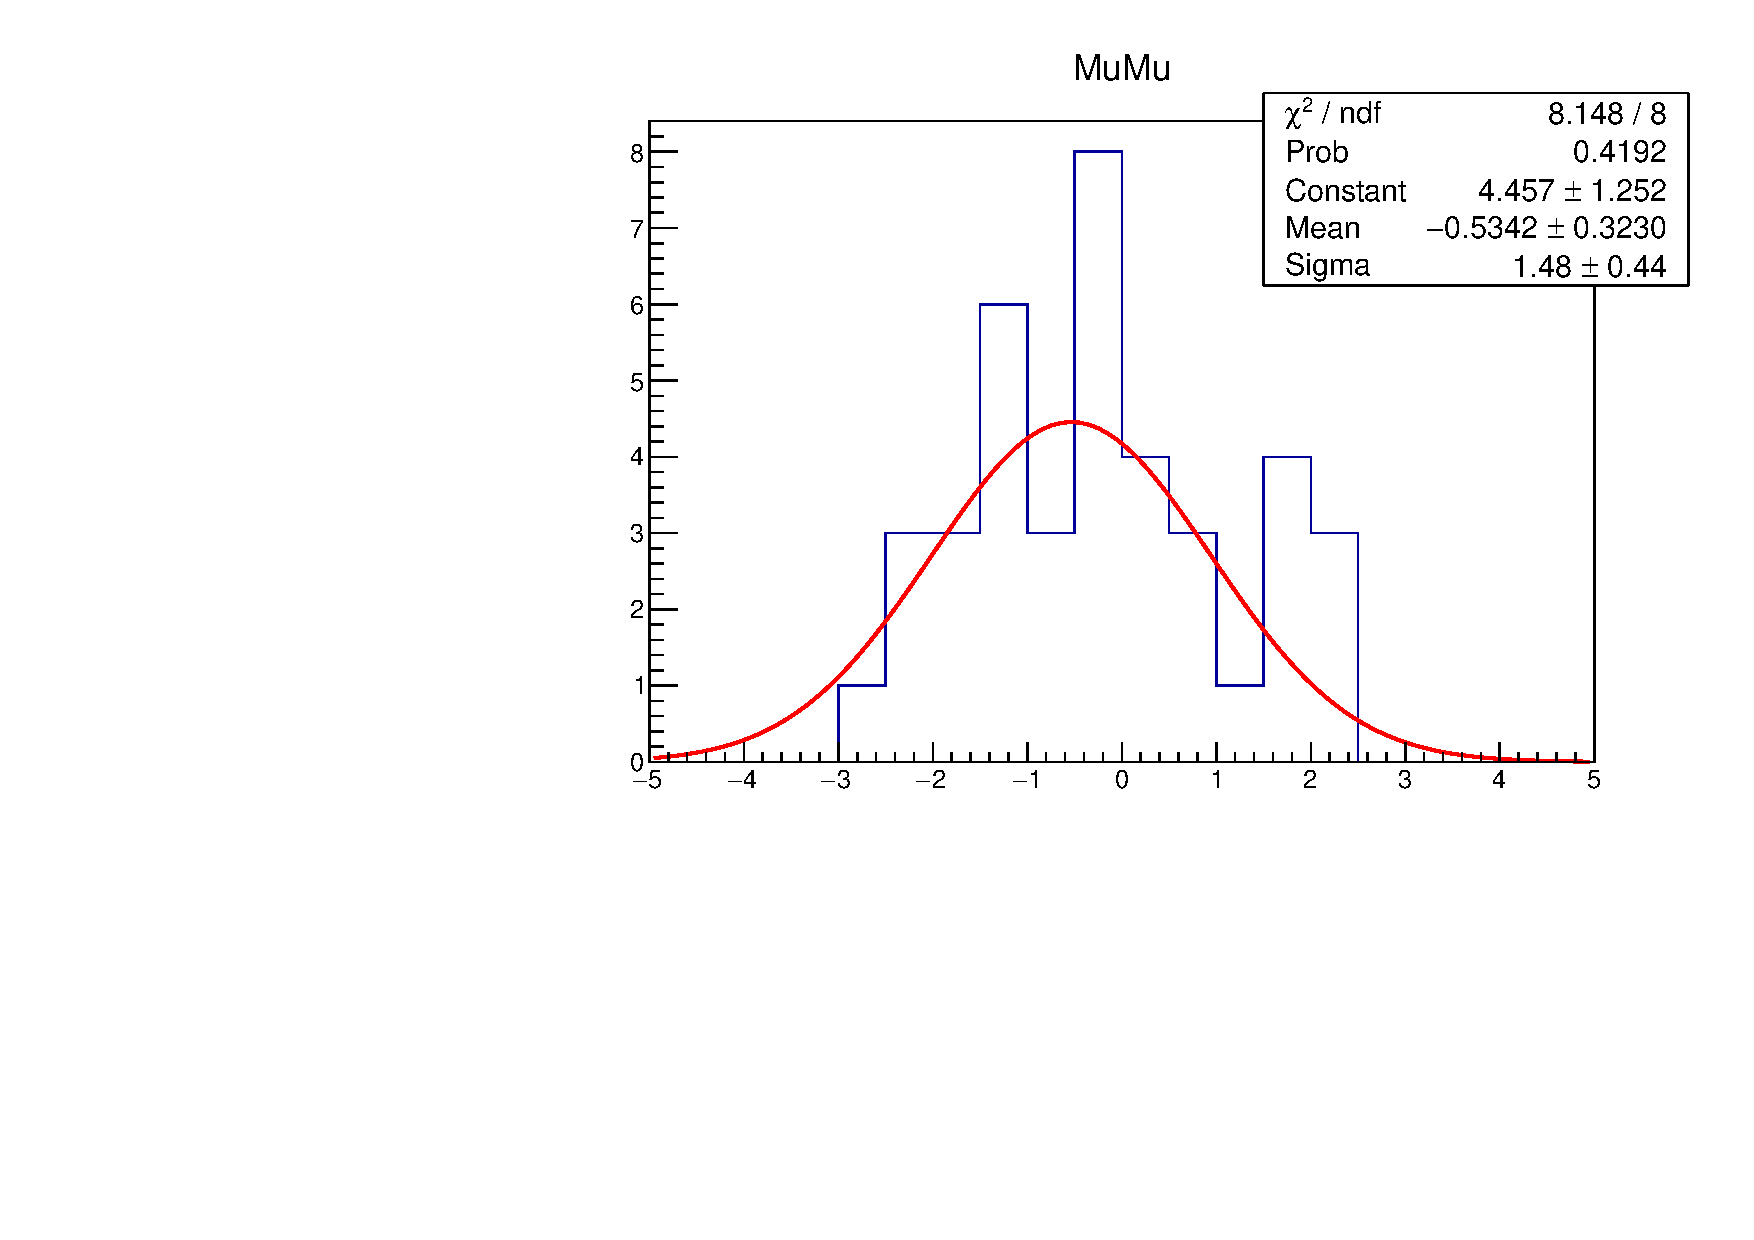
\includegraphics[width=0.5\textwidth]{figures/mhtTemplate/exclusive/MuMu}\\
  \caption{(Left) The best fit value for the linear parameter
    relative to unity in units of the associated statistical
    uncertainty, \ie the statistical ``pull'', as a function of \njet,
    \nb, and \scalht. (Right) The histogram of the pull values.}
  \label{fig:pulls-zinv} 
\end{figure}

The fit information in the figures of App.~\ref{app:mht-zinv} is
summarised in Fig.\ref{fig:pulls-zinv} (left), which shows the best fit
value for the linear parameter (of the first-order orthogonal
polynomial) in units of the
associated statistical uncertainty, \ie the statistical ``pull'', as a
function of \njet, \nb, and \scalht. As for the studies based on the
\mmj sample, the pulls appear not to exhibit any structure as a
function of \njet, \nb, nor \scalht, and are approximately
gaussian-distributed, with a mean and width compatible with zero and
unity, respectively. This indicates that no large, significant bias is
found in the simulation modelling of the \mht variable when events are
categorised by \njet, \scalht, and \nb. (The same conclusion is also
reached without categorising by \nb.)
\begin{figure}[h!]
  \centering
  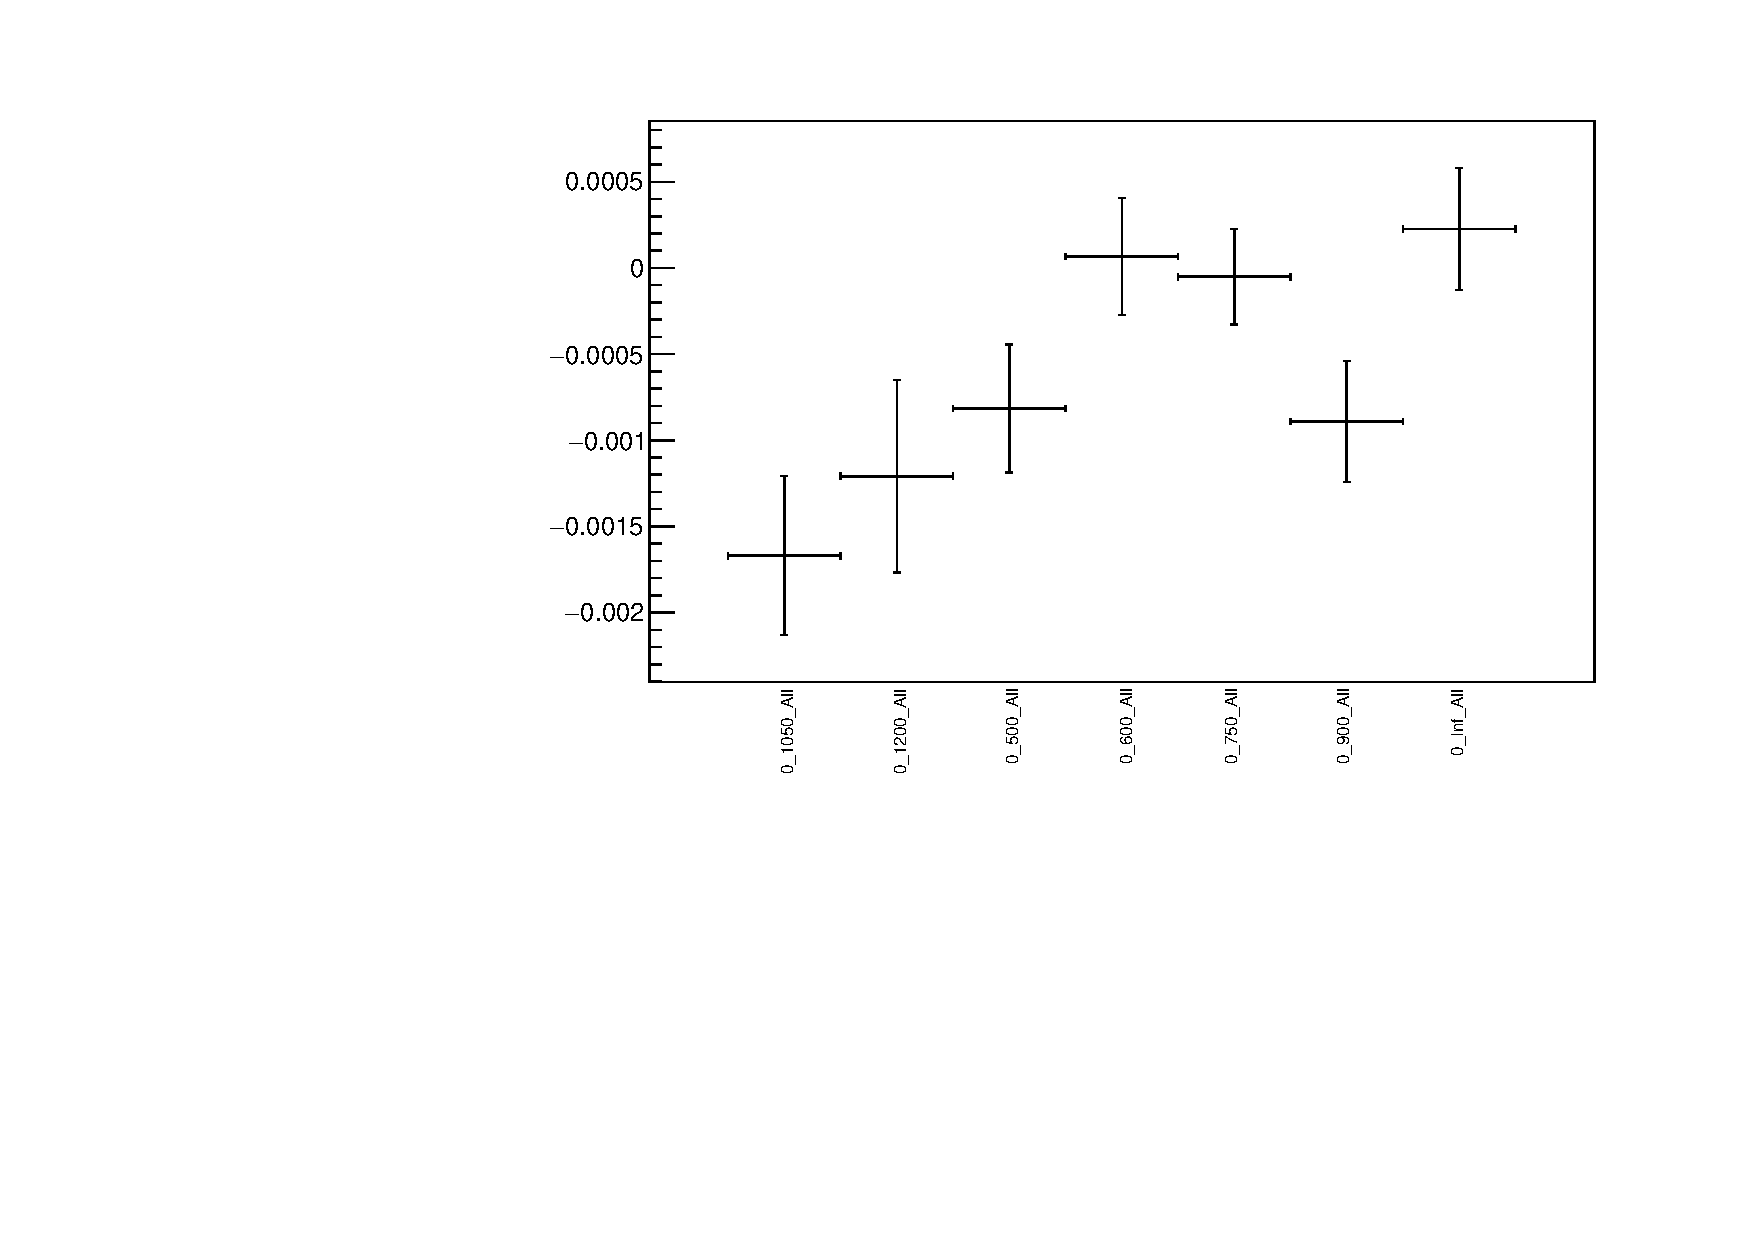
\includegraphics[width=0.5\textwidth]{figures/mhtTemplate/exclusive_corr_njet/MuMu_graph}~
  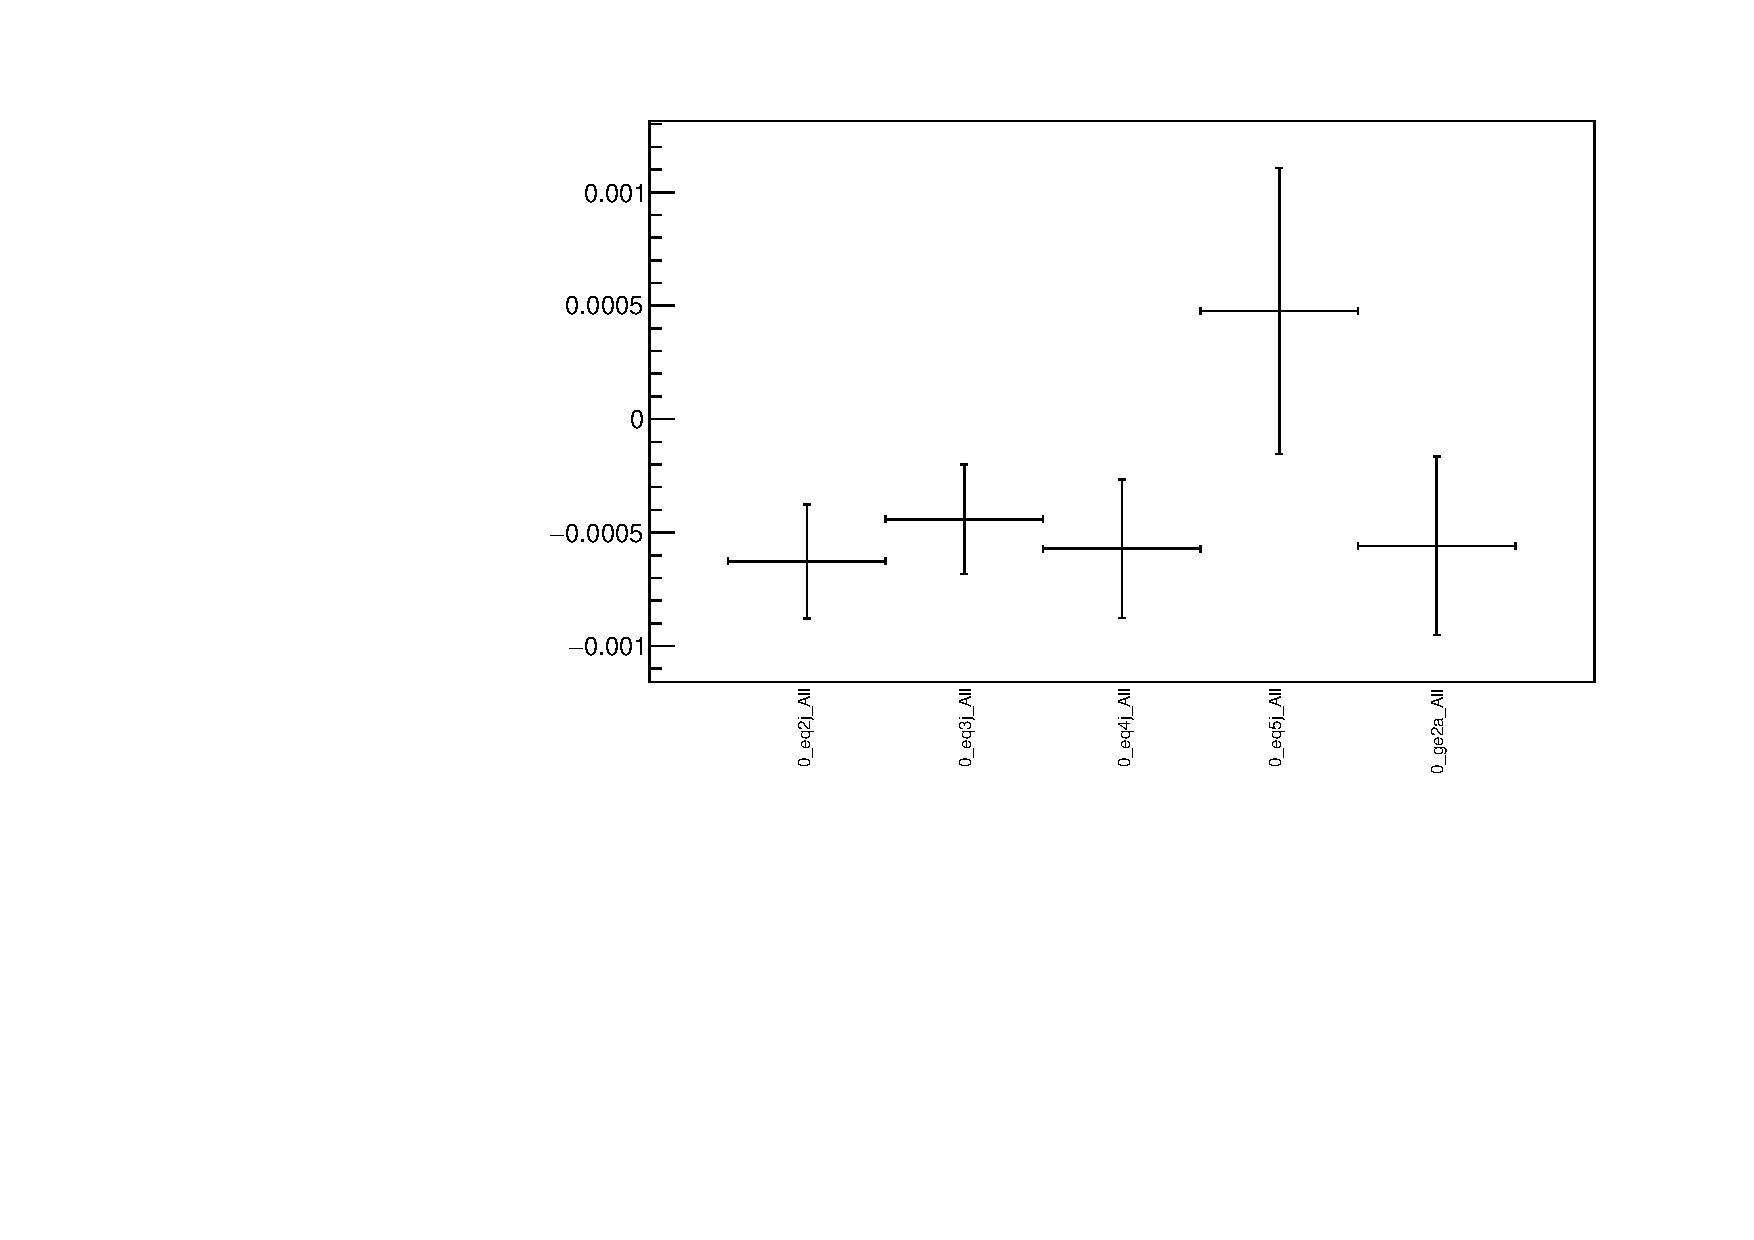
\includegraphics[width=0.5\textwidth]{figures/mhtTemplate/exclusive_corr_ht/MuMu_graph}\\
  \caption{\label{fig:postFitMuMu} Post fit values and uncertainties of
    the linear parameters used to determine the systematics,
    correlated in (left) \njet and (right) \scalht.}
\end{figure}

\begin{figure}[h!]
  \centering
  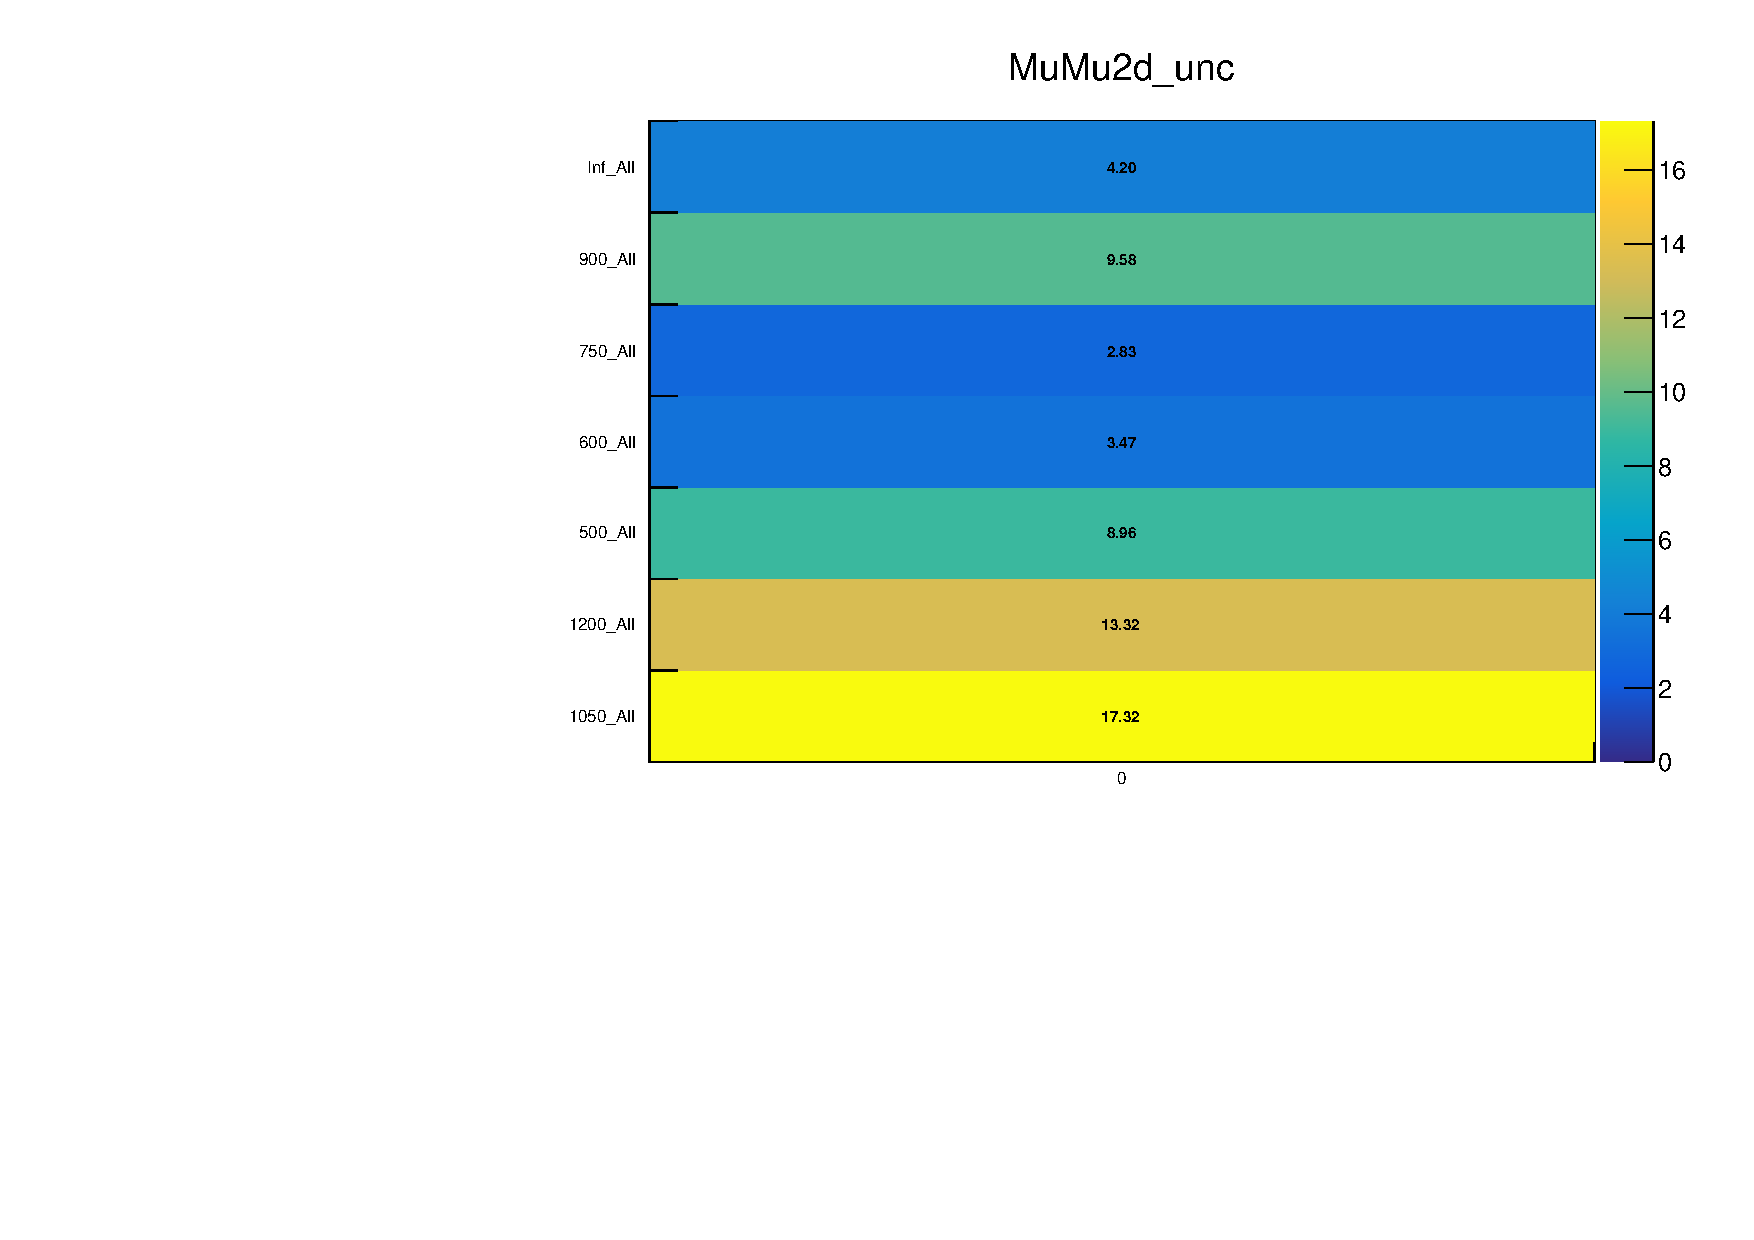
\includegraphics[width=0.5\textwidth]{figures/mhtTemplate/exclusive_corr_njet/MuMu_2D_unc}~
  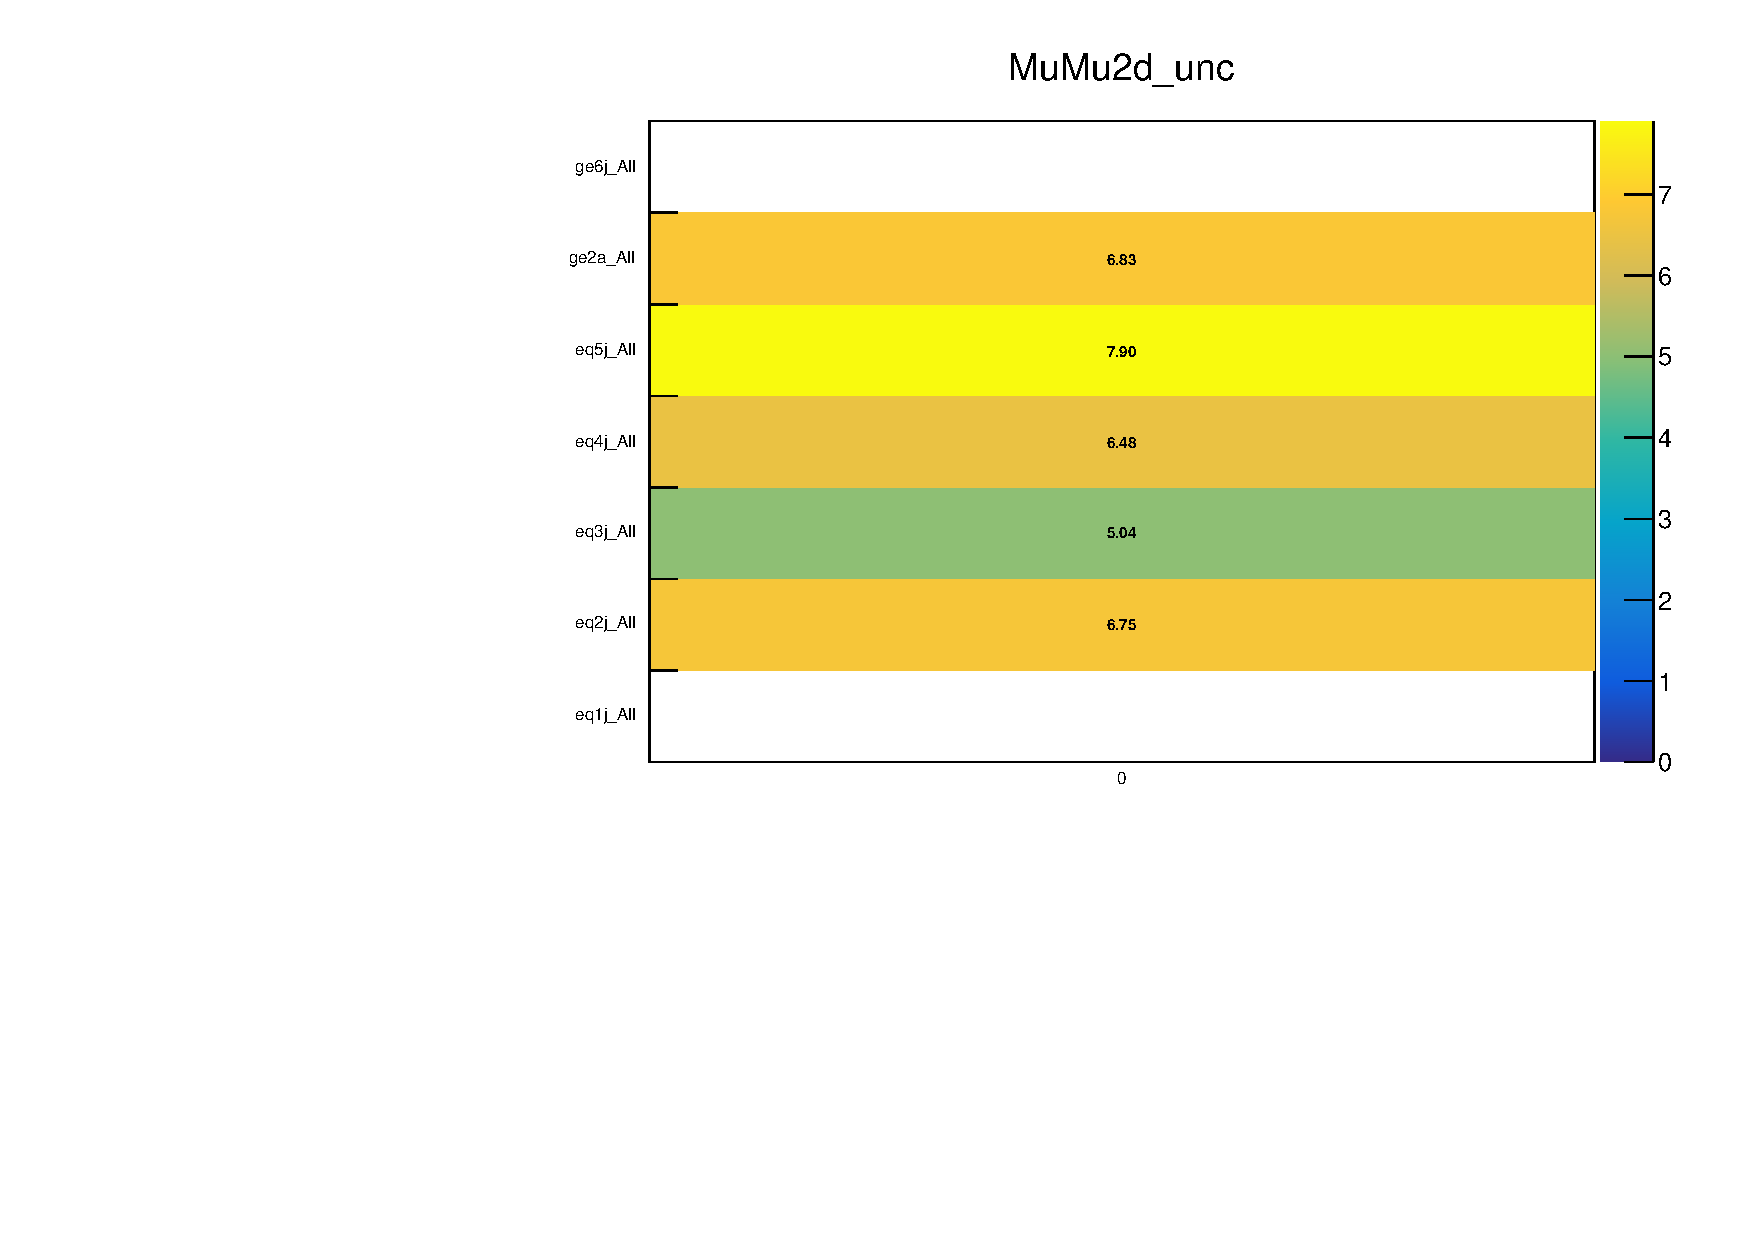
\includegraphics[width=0.5\textwidth]{figures/mhtTemplate/exclusive_corr_ht/MuMu_2D_unc}\\
  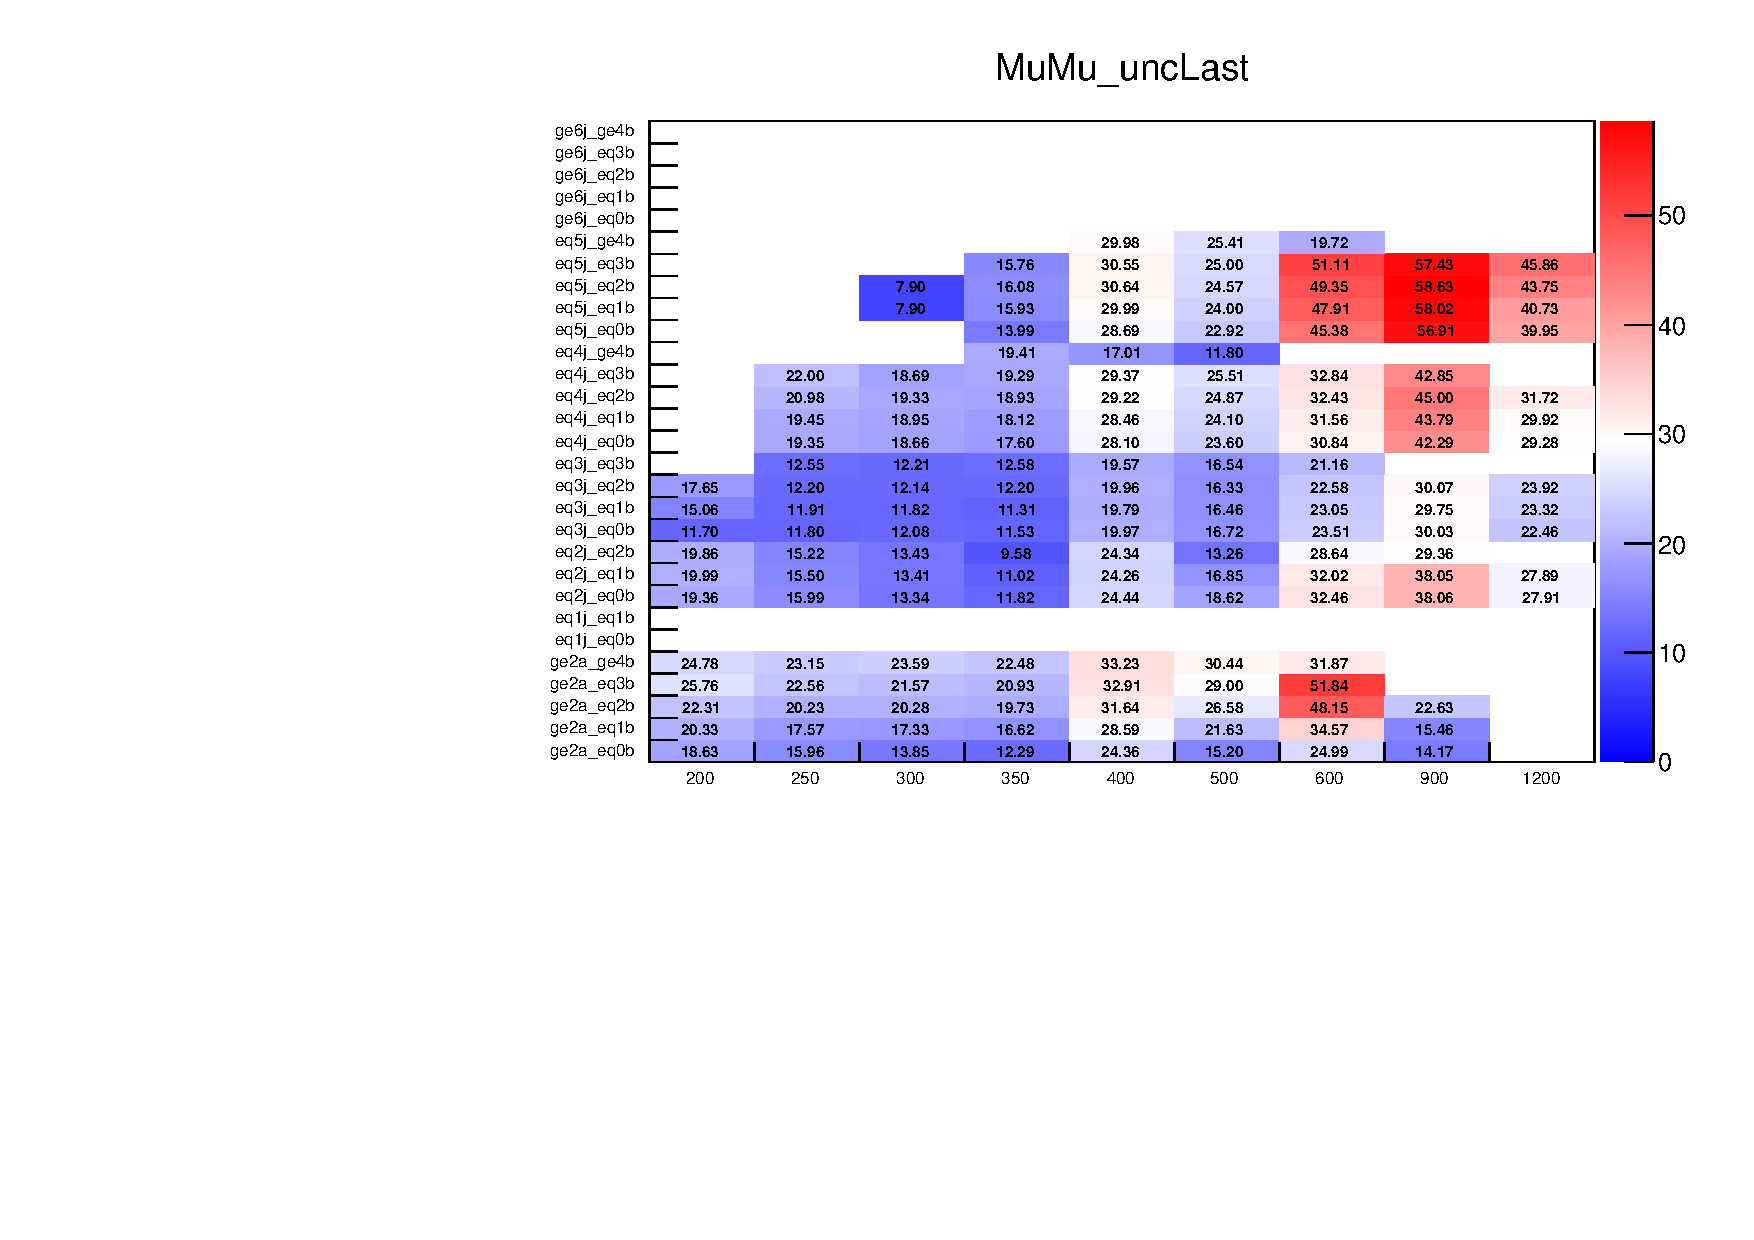
\includegraphics[width=0.5\textwidth]{figures/mhtTemplate/exclusive_corr_ht/MuMu_uncLast}\\
  \caption{\label{fig:postFitErrMuMu} Systematic uncertainties (\%) per
    100\GeV-interval in \mht for effects correlated in (left) \njet
    and (right) \scalht, as determined in the \mmj control
    region. (Bottom) Also shown is the systematic uncertainty (\%) in
    the final open \mht bin for each (\njet, \scalht, \nb) category.}
\end{figure}

The procedure described in Sec.~\ref{sec:mht_syst_mu} is used to
determine the systematic uncertainties in the \mht
modelling. Figure~\ref{fig:postFitMuMu} summarises the post-fit values
and uncertainties of the linear parameters of the orthogonal
polynomials. Figure~\ref{fig:postFitErrMuMu} shows the systematic
uncertainty assumed per 100\GeV-interval in \mht due to effects
correlated in (left) \njet and (right) \scalht, as determined in the
\mmj control region. The values are at the few percent level. Finally,
Figure~\ref{fig:postFitErrMuMu} also shows the systematic uncertainty
in the final open \mht bin for each (\njet, \scalht, \nb) category,
which is typically at the level of 5--20\%.

\subsection{Modelling of the \texorpdfstring{\nb}{Nb} templates}
\label{sec:nb-zinv}

The modelling of the \nb variable for the \znunuj background is
checked with the \mmj sample as a proxy. Uncertainties in the b-tag
scale factor corrections for genuine tags and mistags from the BTV POG
are fully propagated through the method to estimate the \znunuj
background. A binned likelihood fit to the data in the \mmj sample is
performed. The likelihood fit includes several other nuisances related
to known theoretical and experimental sources of uncertainty, as well
as those related to the b-tag scale factors for genuine tags of
b-quark jets (``bsf'') and mistag of light flavour
(``bsfl''). Unconstrained ``rate'' parameters are used per (\njet,
\scalht, $\nb = 0$) or (\njet, \scalht, $\nb \geq 1$) event category
to correct the simulation normalisation to data and the simulation
modelling of the \nb dimension in each (\njet, \scalht, $\nb \geq 1$)
category is fit to data within the statistical uncertainties
associated with the data and smiulated counts. The systematic effects
of the b-tag scale-factor uncertainties are encapsulated by the two
nuisances ``bsf'' and ``bsfl'', which correlate each behaviour across
all (\njet, \scalht) event categories. 

Figure~\ref{fig:btagsfge1b} (top) shows the post-fit nuisances for a
likelihood fit to data in the \mmj control region when the fit is only
given freedom via rate parameters to account for normalisation
differences between simulation and data for the two regions $\nb = 0$
and $\nb \geq 1$. Hence, the fit is sensitive to simulation
mismodelling of the \nb distribution in the region $\nb \geq 1$. The
post-fit nuisance behaviour is consistent with the pre-fit values.

For comparison, Figure~\ref{fig:btagsfge1b} (bottom) shows the same
study, but with only a single rate parameter per (\njet, \scalht)
category, such that the full \nb shape is taken from simulation. Here,
the ``bsf'' and ``bsfl'' nuisances show behaviour that is in tension
with respect to their pre-fit values. The underlying issue in the
mismodelling is unknown, but the behaviour does appear to be dependent
on the run conditions and it has been traced to the run eras B-F, as
summarised in Appendix~\ref{app:nb-zinv}.

In summary, the use of \mmj events subdivided according to $\nb = 0$
and $\nb \geq 1$ appears to fully mitigate the era-dependent issues
and the \nb modelling from simulation appears to be fully adequate for
the purposes of this analysis. 

\begin{figure}[h!]
  \centering
  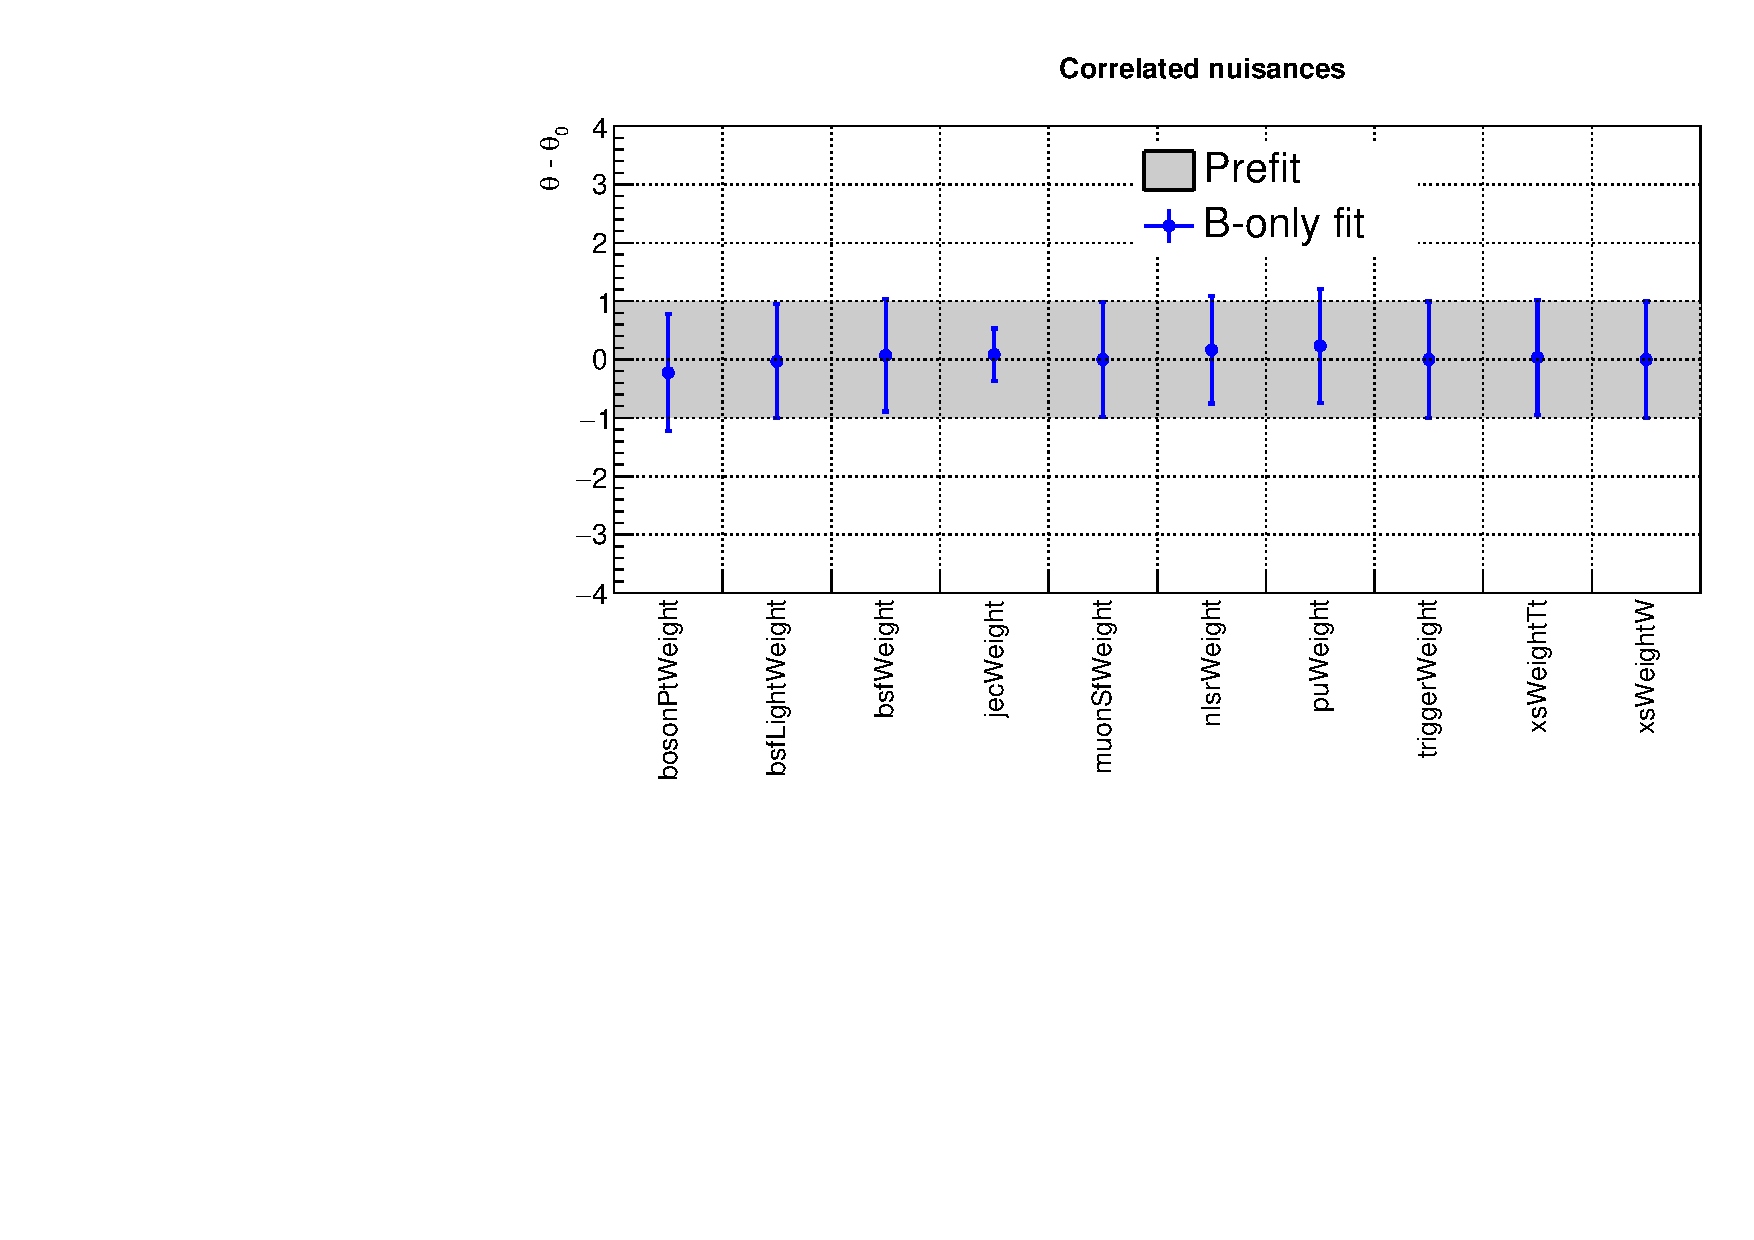
\includegraphics[width=0.6\textwidth]{figures/btag/nuisances/formula/Correlated_nuisances_ge1b}
  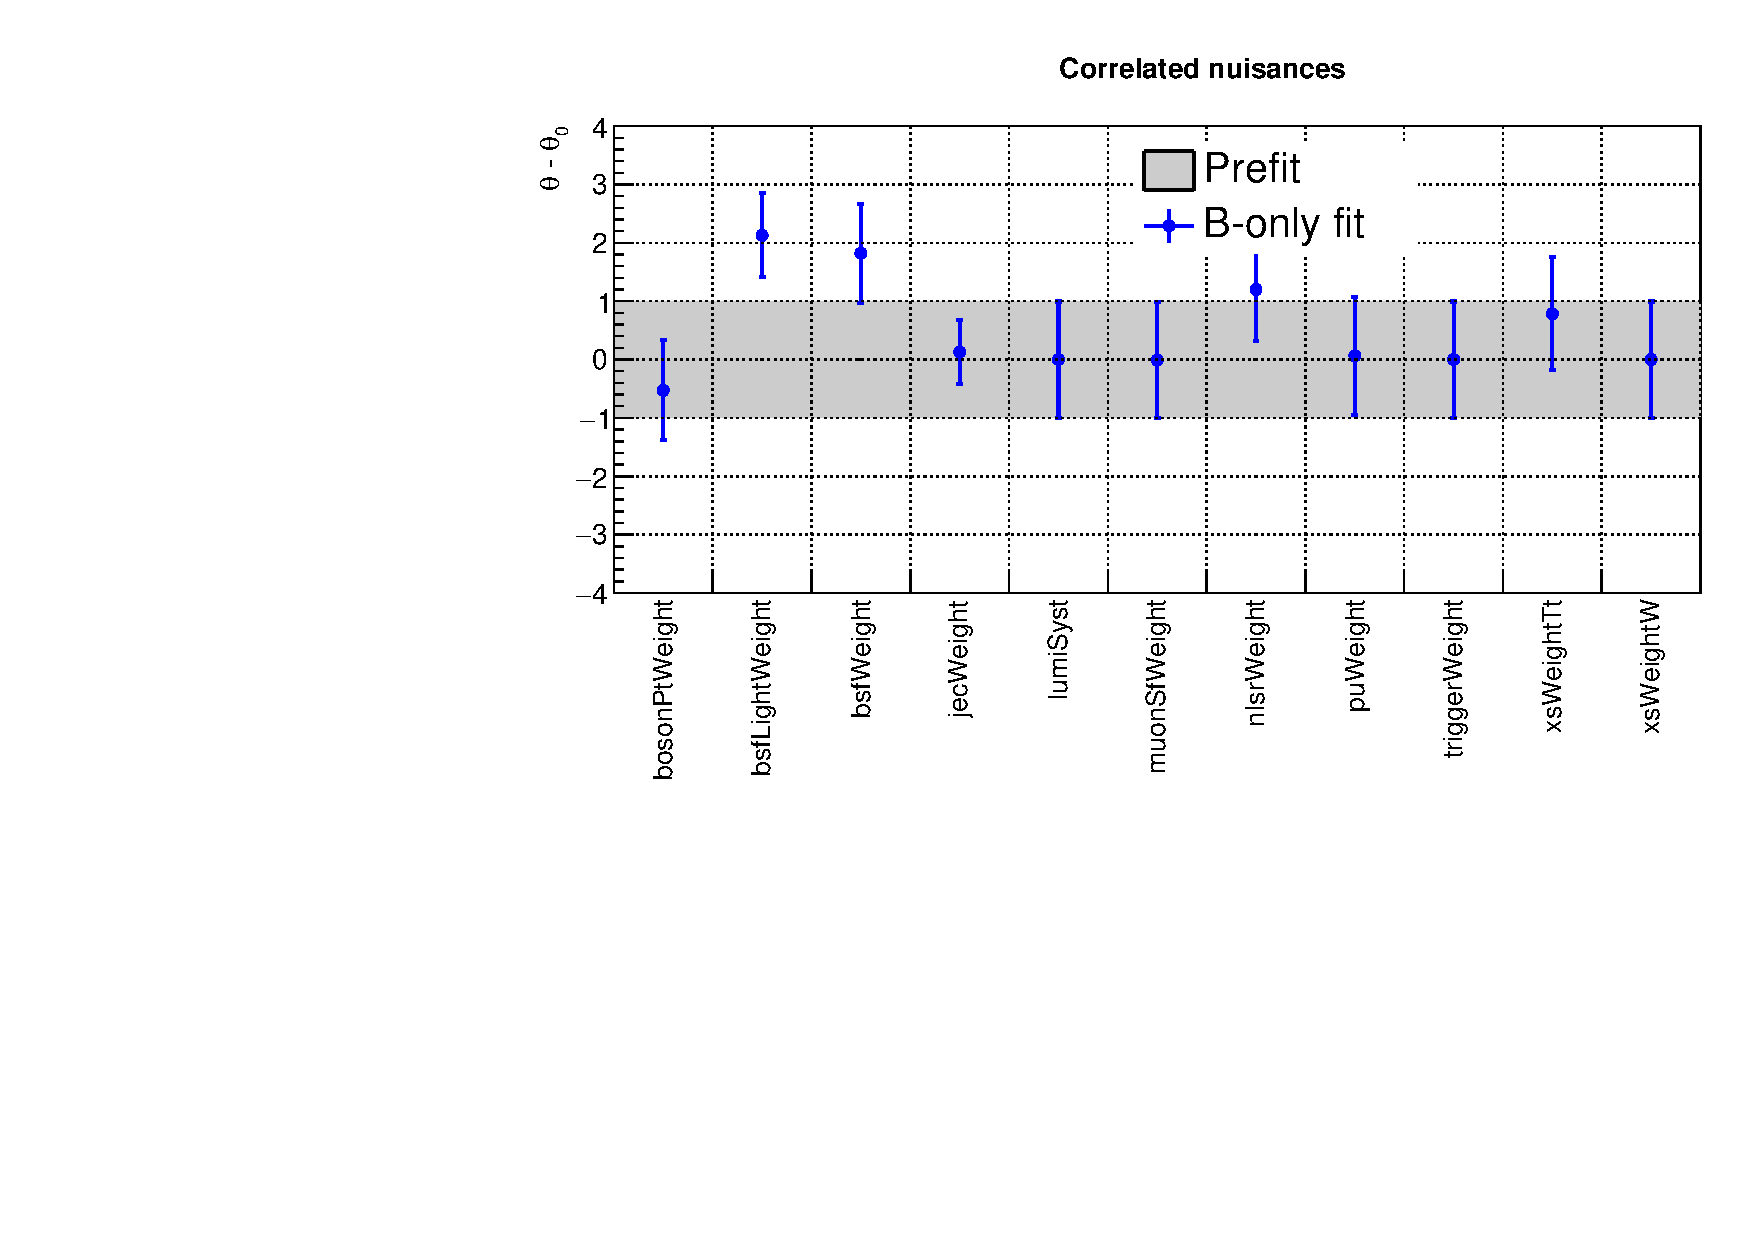
\includegraphics[width=0.6\textwidth]{figures/btag/nuisances/formula/Correlated_nuisances_ge0b}
  \caption{\label{fig:btagsfge1b} Post-fit nuisances of a likelihood
    fit to data in the \mmj control region using the formula method
    for \mmj event counts (top) subdivided according to $\nb = 0$ and
    $\nb \geq 1$, and (bottom) integrated over \nb. }
\end{figure}

